\documentclass[12pt]{article} % use larger type; default would be 10pt

\usepackage{tikz}
\usepackage{pgfplots}
\usetikzlibrary{calc}
\usetikzlibrary{arrows.meta}
\usetikzlibrary{patterns}
        \newcommand\degree[0]{^{\circ}}
\usetikzlibrary{shapes.misc}

\title{Play with TikZ}
\author{Just Us}
%\date{} % Activate to display a given date or no date (if empty),
         % otherwise the current date is printed 

\begin{document}
\maketitle

\section{Chap 6 Review problems}


hp6-sum-23 circle

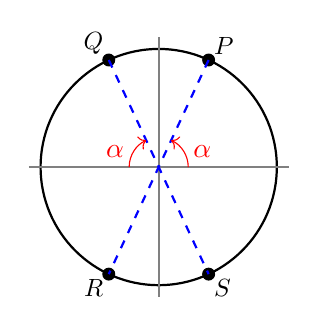
\begin{tikzpicture} [scale=1.5]
\draw[black,thick] (0,0) circle (1cm);
\draw[gray,thick] (-1.1,0)--(1.1,0);
\draw[gray,thick] (0,-1.1)--(0,1.1);
\coordinate (P) at (65:1);
\coordinate (Q) at (115:1);
\coordinate (R) at (245:1);
\coordinate (S) at (295:1);
\filldraw[black] (P) circle (.05cm) node[above right, inner sep=2pt, scale=.9] {$P$};
\filldraw[black] (Q) circle (.05cm) node[above left, inner sep=2pt, scale=.9] {$Q$};
\filldraw[black] (R) circle (.05cm) node[below left, inner sep=2pt, scale=.9] {$R$};
\filldraw[black] (S) circle (.05cm) node[below right, inner sep=2pt, scale=.9] {$S$};
\draw[blue, thick,dashed] (P)--(R);
\draw[blue, thick,dashed] (Q)--(S);
\draw[red,->] (0.25,0) arc(0:65:0.25) node[right, midway]{$\alpha$};
\draw[red,->] (-0.25,0) arc(180:115:0.25) node[left, midway]{$\alpha$};
\end{tikzpicture}
\newline


hp6-rev-41ans sine and cosine

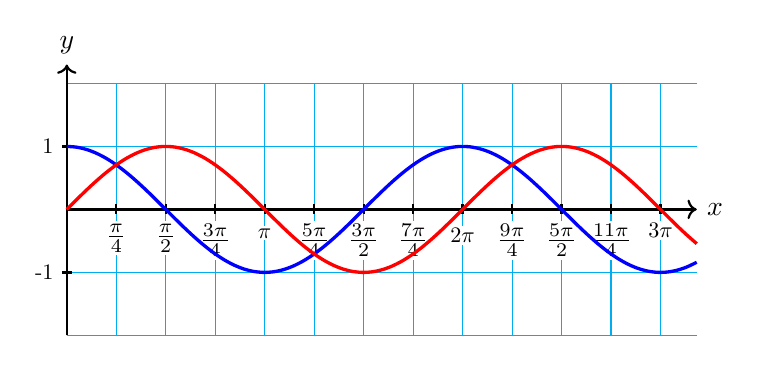
\begin{tikzpicture} [scale=.8]
\draw[cyan] (0,-2) grid[xstep=pi/4, ystep=1] (10,2);
\draw[black,thick,->](0,0)--(10.,0) node[right]{$x$};
\draw[black,thick,->](0,-2)--(0,2.3) node[above]{$y$};
\foreach \y in {-1,1} \draw[black,thick] (0.08,\y)--++(-.16,0) node[left, scale=.8]{\y};
\draw[black,thick] (pi/4,.08)--++(0,-.16) node[below, yshift=-2, fill=white, inner sep=1] {$ \frac{\pi}{4}$};
\draw[black,thick] (pi/2,.08)--++(0,-.16) node[below, yshift=-2, fill=white, inner sep=1] {$ \frac{\pi}{2}$};
\draw[black,thick] (3*pi/4,.08)--++(0,-.16) node[below, yshift=-2, fill=white, inner sep=1] {$ \frac{3\pi}{4}$};
\draw[black,thick] (pi,.08)--++(0,-.16) node[below, yshift=-4, fill=white, inner sep=1, scale=.8] {$ \pi$};
\draw[black,thick] (5*pi/4,.08)--++(0,-.16) node[below, yshift=-2, fill=white, inner sep=1] {$ \frac{5\pi}{4}$};
\draw[black,thick] (3*pi/2,.08)--++(0,-.16) node[below, yshift=-2, fill=white, inner sep=1] {$ \frac{3\pi}{2}$};
\draw[black,thick] (7*pi/4,.08)--++(0,-.16) node[below, yshift=-2, fill=white, inner sep=1] {$ \frac{7\pi}{4}$};
\draw[black,thick] (2*pi,.08)--++(0,-.16) node[below, yshift=-4, fill=white, inner sep=1, scale=.8] {$ 2\pi$};
\draw[black,thick] (9*pi/4,.08)--++(0,-.16) node[below, yshift=-2, fill=white, inner sep=1] {$ \frac{9\pi}{4}$};
\draw[black,thick] (5*pi/2,.08)--++(0,-.16) node[below, yshift=-2, fill=white, inner sep=1] {$ \frac{5\pi}{2}$};
\draw[black,thick] (11*pi/4,.08)--++(0,-.16) node[below, yshift=-2, fill=white, inner sep=1] {$ \frac{11\pi}{4}$};
\draw[black,thick] (3*pi,.08)--++(0,-.16) node[below, yshift=-2, fill=white, inner sep=1, scale=.8] {$ 3\pi$};
\draw[samples=65, domain=0:10, variable=\x, smooth,blue, very thick] plot(\x,{cos(deg(\x))});
\draw[samples=65, domain=0:10, variable=\x, smooth, red, very thick] plot(\x,{sin(deg(\x))});
\end{tikzpicture}
\newline


hp6-rev-43ansa
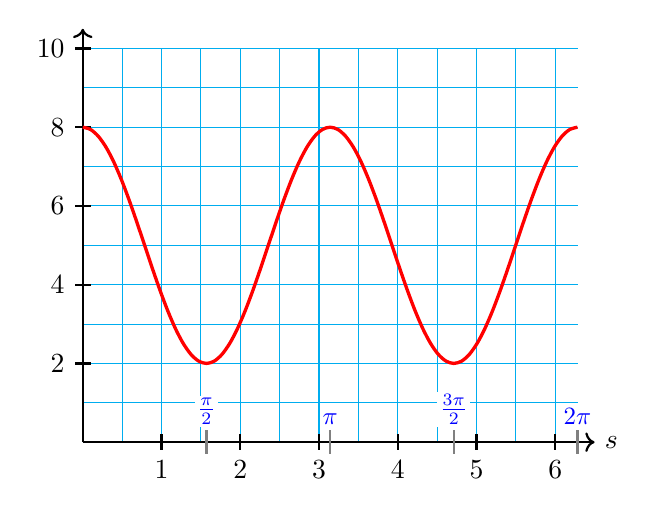
\begin{tikzpicture} [yscale=.5]
\draw[cyan] (0,0) grid[xstep=1/2] (2*pi, 10);
\draw[black,thick,->] (0,0)--(6.5,0) node[right]{$s$};
\draw[black,thick,->] (0,0)--(0,10.5) ;
\foreach \x in {1,2, ...,6} \draw[black,thick] (\x,.2)--++(0,-.4) node[below]{\x};
\foreach \y in {2, 4, ...,10} \draw[black,thick] (0.1,\y)--++(-.2,0) node[left]{\y};
\draw[gray,thick] (pi/2,-.3)--++(0,.6) node[above, yshift=1, fill=white, inner sep=1, text=blue, scale=.9]{$\frac{\pi}{2}$};
\draw[gray,thick] (pi,-.3)--++(0,.6) node[above, yshift=1, fill=white, inner sep=1, text=blue, scale=.9]{$\pi$};
\draw[gray,thick] (2*pi,-.3)--++(0,.6) node[above, yshift=1, fill=white, inner sep=1, text=blue, scale=.9]{$2\pi$};
\draw[gray,thick] (3*pi/2,-.3)--++(0,.6) node[above, yshift=1, fill=white, inner sep=1, text=blue, scale=.9]{$\frac{3\pi}{2}$};
\draw[samples=65,domain=0:2*pi,smooth,variable=\x,red,very thick] plot ({\x},{5+3* cos( deg(2*\x) )});\end{tikzpicture}
\newline


hp6-rev-43ansb
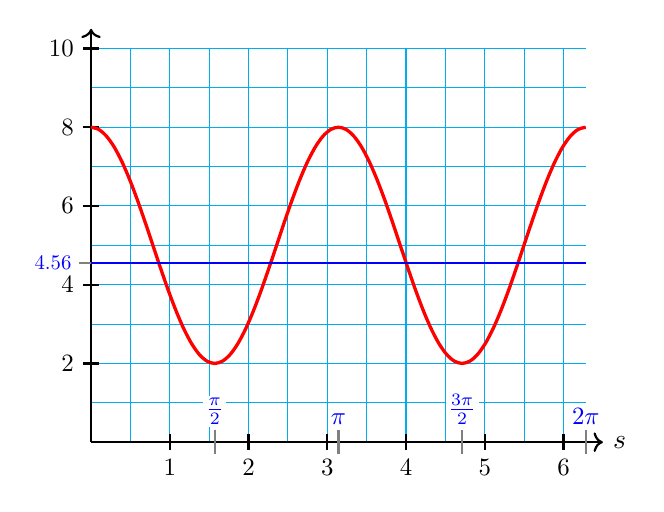
\begin{tikzpicture} [yscale=.5]
\draw[cyan] (0,0) grid[xstep=1/2] (2*pi, 10);
\draw[black,thick,->] (0,0)--(6.5,0) node[right]{$s$};
\draw[black,thick,->] (0,0)--(0,10.5) ;
\foreach \x in {1,2, ...,6} \draw[black,thick] (\x,.2)--++(0,-.4) node[below, scale=.9]{\x};
\foreach \y in {2, 4, ...,10} \draw[black,thick] (0.1,\y)--++(-.2,0) node[left, scale=.9]{\y};
\draw[gray,thick] (pi/2,-.3)--++(0,.6) node[above, yshift=1, fill=white, inner sep=1, text=blue, scale=.9]{$\frac{\pi}{2}$};
\draw[gray,thick] (pi,-.3)--++(0,.6) node[above, yshift=1, fill=white, inner sep=1, text=blue, scale=.9]{$\pi$};
\draw[gray,thick] (2*pi,-.3)--++(0,.6) node[above, yshift=1, fill=white, inner sep=1, text=blue, scale=.9]{$2\pi$};
\draw[gray,thick] (3*pi/2,-.3)--++(0,.6) node[above, yshift=1, fill=white, inner sep=1, text=blue, scale=.9]{$\frac{3\pi}{2}$};
\draw[samples=65,domain=0:2*pi,smooth,variable=\x,red,very thick] plot ({\x},{5+3* cos( deg(2*\x) )});
\draw[gray,thick] (0,4.56)--++(-.15,0) node[left, text=blue, scale=0.75]{4.56};
\draw[blue,thick] (0,4.56) -- ++(2*pi,0);
\end{tikzpicture}
\newline


hp6-rev-45ansa
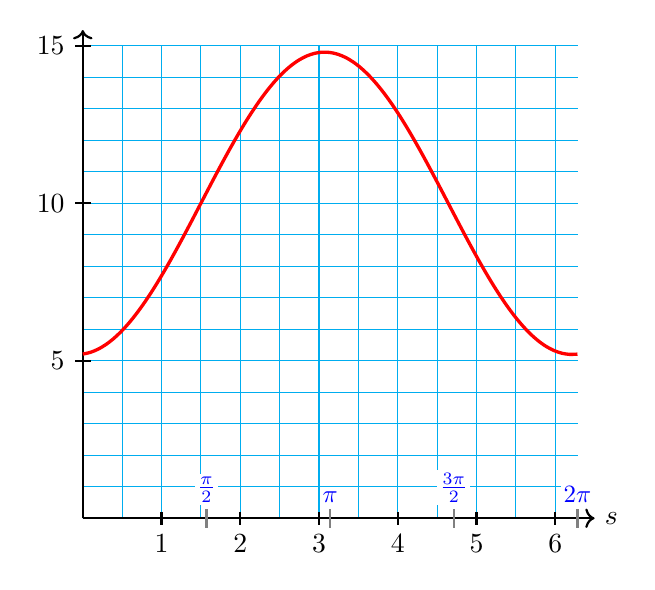
\begin{tikzpicture} [yscale=.4]
\draw[cyan] (0,0) grid[xstep=1/2] (2*pi, 15);
\draw[black,thick,->] (0,0)--(6.5,0) node[right]{$s$};
\draw[black,thick,->] (0,0)--(0,15.5) ;
\foreach \x in {1,2, ...,6} \draw[black,thick] (\x,.2)--++(0,-.4) node[below]{\x};
\foreach \y in {5,10,15} \draw[black,thick] (0.1,\y)--++(-.2,0) node[left]{\y};
\draw[gray,thick] (pi/2,-.3)--++(0,.6) node[above, yshift=1, fill=white, inner sep=1, text=blue, scale=.9]{$\frac{\pi}{2}$};
\draw[gray,thick] (pi,-.3)--++(0,.6) node[above, yshift=1, fill=white, inner sep=1, text=blue, scale=.9]{$\pi$};
\draw[gray,thick] (2*pi,-.3)--++(0,.6) node[above, yshift=1, fill=white, inner sep=1, text=blue, scale=.9]{$2\pi$};
\draw[gray,thick] (3*pi/2,-.3)--++(0,.6) node[above, yshift=1, fill=white, inner sep=1, text=blue, scale=.9]{$\frac{3\pi}{2}$};
\draw[samples=65,domain=0:2*pi,smooth,variable=\x,red,very thick] plot ({\x},{10+4.8* sin( deg(\x-1.5) )});
\end{tikzpicture}
\newline


hp6-rev-45ansb
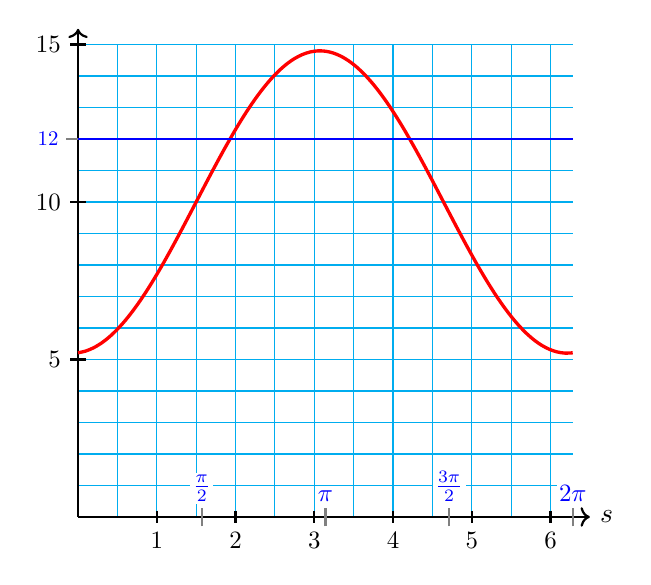
\begin{tikzpicture} [yscale=.4]
\draw[cyan] (0,0) grid[xstep=1/2] (2*pi, 15);
\draw[black,thick,->] (0,0)--(6.5,0) node[right]{$s$};
\draw[black,thick,->] (0,0)--(0,15.5) ;
\foreach \x in {1,2, ...,6} \draw[black,thick] (\x,.2)--++(0,-.4) node[below, scale=.9]{\x};
\foreach \y in {5,10,15} \draw[black,thick] (0.1,\y)--++(-.2,0) node[left, scale=.9]{\y};
\draw[gray,thick] (pi/2,-.3)--++(0,.6) node[above, yshift=1, fill=white, inner sep=1, text=blue, scale=.9]{$\frac{\pi}{2}$};
\draw[gray,thick] (pi,-.3)--++(0,.6) node[above, yshift=1, fill=white, inner sep=1, text=blue, scale=.9]{$\pi$};
\draw[gray,thick] (2*pi,-.3)--++(0,.6) node[above, yshift=1, fill=white, inner sep=1, text=blue, scale=.9]{$2\pi$};
\draw[gray,thick] (3*pi/2,-.3)--++(0,.6) node[above, yshift=1, fill=white, inner sep=1, text=blue, scale=.9]{$\frac{3\pi}{2}$};
\draw[samples=65,domain=0:2*pi,smooth,variable=\x,red,very thick] plot ({\x},{10+4.8* sin( deg(\x-1.5) )});
\draw[gray,thick] (0,12)--++(-.15,0) node[left, text=blue, scale=0.75]{12};
\draw[blue,thick] (0,12) -- ++(2*pi,0);
\end{tikzpicture}
\newline


hp6-rev-63ans parabola

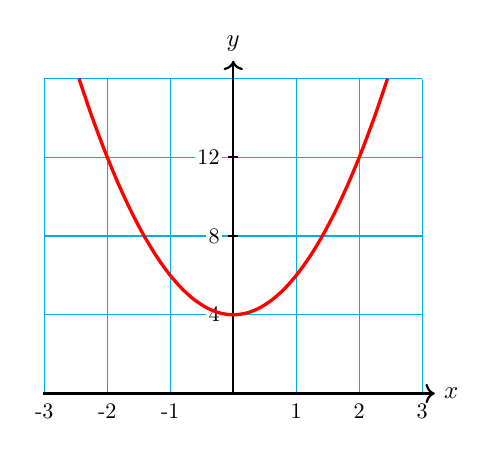
\begin{tikzpicture} [xscale=.8,yscale=1/4]
\draw[cyan] (-3,0) grid[ystep=4] (3,16);
\draw[black,thick,->] (-3,0)--(3.2,0) node[right, scale=.9]{$x$};
\draw[black,thick,->] (0,0)--(0,16.9) node[above, scale=.9]{$y$};
\foreach \x in {-3,-2,-1,1,2,3} \draw[black,thick] (\x,.1)--++(0,-.2) node[below, scale=.8] {\x};
\foreach \y in {4,8,12} \draw[black,thick] (.08,\y)--++(-.16,0) node[left, xshift=-2, fill=white, inner sep=1, scale=.8] {\y};
\draw[,domain=-sqrt(6):sqrt(6),smooth,variable=\x,red,very thick] plot ({\x},{2*(\x)^2+4 });
\end{tikzpicture}
\newline


hp6-rev-65ans semicircle
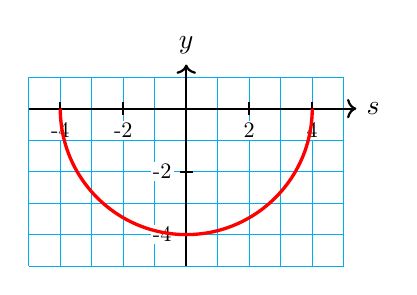
\begin{tikzpicture} [scale=.4]
\draw[cyan] (-5,-5) grid (5,1);
\draw[black,thick,->] (-5,0)--(5.4,0) node[right]{$s$};
\draw[black,thick,->] (0,-5)--(0,1.4) node[above]{$y$};
\foreach \i in {2,4} {
 \draw[black,thick] (\i,0.2)--++(0,-.4) node[below, yshift=-2, fill=white, inner sep=1pt, scale=.8] {\i};
 \draw[black,thick] (-\i,0.2)--++(0,-.4) node[below, yshift=-2, fill=white, inner sep=1pt, scale=.8] {-\i};
 \draw[black,thick] (0.2,-\i)--++(-0.4,0) node[left, xshift=-2, fill=white, inner sep=1pt, scale=.8] {-\i};
};
\draw[red,very thick] (4,0) arc (0:-180:4);
\end{tikzpicture}
\newline



\end{document}
